% \chapter{Pr\'{e}sentation des problèmes}

% TODO Introduction avec définition général des problèmes d'ordonnancement et présentation des
% différentes possibilités + Introduction du modèle
% TODO Présentation de l'interval Scheduling et du problème de réservation de l'hotel
% TODO Présentation du modèle de notation à trois champs

% <<< Previous Intro : Ordonnancement
%\section{Introduction}
%\subsection{L'ordonnancement}
%
%L'ordonnancement est un processus décisionnel très répandu utilisé très régulièrement par
%les entreprises, les industries et même les particuliers.  Il s'occupe de répartir une certaine quantité de
%ressources entre différentes tâches s'étalant sur une période donnée et s'attache en général à
%optimiser un ou plusieurs objectifs. Ainsi un emploi du temps est une forme d'ordonnancement,
%affectant du temps à un ensemble de tâches à réaliser.
%
%Ainsi l'étude de la théorie de l'ordonnancement, de par son fort potentiel applicatif, a été très
%largement étudiée, ce qui a donné naissance à une multitude de problèmes. Dans la littérature, les
%problème d'ordonnancement de décrivent généralement de la manière suivante : un ensemble de tâches
%$\mathcal{T} = \{T_1, T_2, \dots, T_n\}$, un ensemble de machines $\mathcal{M} = \{M_1, M_2, \dots,
%M_k\}$. Un ordonnancement consiste donc à affecter l'ensemble des tâches à l'ensemble des machines
%en respectant des contraintes imposées. Deux de ces contraintes, sûrement les plus répandues dans les
%problèmes d'ordonnancement, imposent qu'à chaque instant, chaque machine n'est capable de d'exécuter au
%plus qu'une seule tâche et que chaque tâche n'est exécutée que par une seule machine.
%
%Il est possible de caractériser l'ensemble des machines prises en compte, ainsi ces dernières
%peuvent être parallèles, c'est-à-dire exécutant les mêmes fonctions, soit dédiées, dans ce cas elles
%sont spécialisées dans le traitement de certaines tâches. Nous ne nous intéresserons uniquement au
%premier cas. On peut aller plus loin dans la caractérisation des machines en faisant une distinction
%basée sur la vitesse de traitement. Si chaque tâche s'exécute à la même vitesse sur chacune des
%machines, elles sont dites identiques, si les vitesses de traitement diffèrent, mais chaque vitesse
%$b_i$ (facteur d'accélération de traitement de la tâche) des machines est constante et ne dépend
%pas de la tâche à exécuter, les machines sont dites uniformes. Enfin, si la vitesse de traitement
%d'une tâche dépend de cette tâche les machines sont alors appelées générales.
%
%% Références de bouquins traitant le sujet avec plus de précision.
%
%%Choses à faire :
%%\begin{itemize}
%%    \item présentation du domaine
%%    \item définition d'un ordonnancement
%%    \item introduction à la notation à trois champs
%%\end{itemize}
%
%De la même manière, il est possible d'imposer des contraintes sur la manière d'exécuter les tâches,
%on peut par exemple autoriser (ou interdire) la préemption des tâches, i.e. autoriser l'interruption
%de l'exécution d'une tâche à n'importe quel moment et son exécution peut être reprise à n'importe
%quel instant, un ordonnancement autorisant (resp. interdisant) la préemption est dit préemptif
%(resp. non-préemptif). On peut aussi autoriser la duplication des tâches, afin de, par exemple,
%réduire l'influence des délais de communication entre machines lorsque ceux ci sont définis, en
%produisant des copies sur différentes machines.
%On peut trouver des contraintes de précédence entre les tâches, ainsi $t_i
%\prec t_j$ signifie que la tâche $t_j$ ne peut commencer qu'une fois la tâche $t_i$ terminée. Les
%tâches soumises à des relations de précédence sont représentées par un graphe orienté dans lequel
%les sommets correspondent aux taches et les arêtes aux relations de précédence.
%
%
%\subsection{Notation à trois champs}
%
%La grande diversité de problèmes couverts par l'ordonnancement a conduit à la mise en place d'une
%notation normalisée permettant de classifier les schémas. Nous décrivons donc, de manière non
%exhaustive, la notation introduite par Graham~\cite{graham} et al. et Bla\.{z}evicz et
%al.~\cite{blazewicz}. Il s'agit d'une
%notation utilisant trois paramètres $\alpha, \beta$ et $\gamma$ permettant de synthétiser la
%description des problèmes d'ordonnancement statique.
%
%\begin{enumerate}
%    \item le paramètre $\alpha = \alpha_1(\alpha_2),\ \alpha \in \{P, \bar{P}, P_m, \dots\} ,\
%            \alpha_2 \in \{P, \bar{P}, P_m, Q, R, \dots\}$\footnote{Notons que certaines combinaisons
%        peuvent n'avoir aucun sens.} définit les caractéristiques des machines considérées.
%        \begin{itemize}
%            \item si $\alpha_i = P$ avec $i \in \{1, 2\}$, alors les machines sont identiques et
%                leur nombre est une entrée du problème,
%            \item si $\alpha_i = \bar{P}$, alors les machines sont identiques mais leur nombre est
%                non borné,
%            \item si $\alpha_i = P_m$, alors les machines sont identiques et leur nombre $m$ est
%                fixé,
%            \item si $\alpha_2 = Q$, les machines sont uniformes,
%            \item si $\alpha_2 = R$ alors les machines sont générales.
%        \end{itemize}
%    \item le paramètre $\beta$ définit les caractéristiques d'exécution des tâches c'est-à-dire le
%        graphe de précédence, les coûts de communication, les temps d'exécution, la possibilité ou
%        non de duplication des tâches et l'autorisation ou non de la préemption.
%        Le paramètre $\beta$ peut alors s'écrire sous la forme $\beta =
%        \beta_1\beta_2\beta_3\beta_4\beta_5$ avec :
%        \begin{itemize}[label=$\circ$]
%            \item $\beta_1 \in \{$prec, intervalle, arbre, $\dots, . \}$
%                \begin{itemize}
%                    \item $\beta_1 =$ prec : le graphe est quelconque
%                    \item $\beta_1 =$ intervalle : le graphe est un graphe d'intervalles
%                    \item $\beta_1 =$ arbre : le graphe est un arbre
%                    \item[$\vdots$] ~
%                    \item $\beta_1 =$ . les tâches sont indépendantes
%                \end{itemize}
%            \item $\beta_2 \in \{$com, $c_{jk}, c, .\}$
%                \begin{itemize}
%                    \item $\beta_2 =$ com : les temps de communication sont donnés par le graphe
%                    \item $\beta_2 = c_{jk}$ : les temps de communication sont donnés par une
%                        matrice de $c_{jk}$ représentant le délai de communication entre la tâche
%                        $j$ et la tâche $k$
%                    \item $\beta_2 = c$ : les temps de communication sont constant et égaux entre
%                        chaque paire de tâches
%                    \item $\beta_2 = .$ : il n'y a pas de temps de communication
%                \end{itemize}
%            \item $\beta_3 \in \{p_j, .\}$
%                \begin{itemize}
%                    \item $\beta_3 = p_j = 1$ : toutes les tâches on une durée unitaire
%                    \item $\beta_3 = .$ : les durées d'exécution sont définies par le graphe
%                \end{itemize}
%            \item $\beta_4 \in \{$dup, $. \}$
%                \begin{itemize}
%                    \item $\beta_4 =$ dup : la duplication est autorisée
%                    \item $\beta_4 = .$ : la duplication est interdite
%                \end{itemize}
%            \item $\beta_5 \in \{$pmpt, $. \}$
%                \begin{itemize}
%                    \item $\beta_5 =$ pmpt : la préemption est autorisée
%                    \item $\beta_5 = .$ : la préemption est interdite
%                \end{itemize}
%        \end{itemize}
%    \item le paramètre $\gamma$ définit la fonction objectif à optimiser.
%\end{enumerate}
%% 
%
% >>>
\section{Introduction}

La théorie de l'ordonnancement est une branche non négligeable de l'informatique couvrant un très
grand nombre de problèmes permettant la modélisation d'applications pratiques. Ainsi, des
problématiques aussi diverses que la planification de prises de photographies par satellite,
l'agencement spatial de marchandises dans un entrepôt ou la planification d'une chaîne de production
peuvent être représentées à l'aide de ces problèmes informatiques. Il n'est donc pas étonnant de
disposer à ce sujet d'une littérature fournie, détaillant nombre de déclinaisons de problèmes
considérés classiques. Cette étude bibliographique, préliminaire au stage, s'inscrit dans cette
démarche et cherche à définir le contexte et les bases nécessaires à l'introduction d'une variante
d'un problème d'ordonnancement très étudié que l'on appelle \isched.

\subsection{Description des problèmes d'ordonnancement}

Nous utiliserons au cours de cette partie les notations communément utilisées pour définir de
manière générale les problèmes d'ordonnancement. Nous serons amenés à définir et utiliser des
notations plus spécifiques au problème considéré.

D'ordinaire, les problèmes d'ordonnancement sont définis par un ensemble de $n$ tâches $\mathcal{T} =
\{T_1, T_2, \dots, T_n\}$ et par un ensemble de $m$ processeurs\footnote{On les appelle aussi des
machines.} $\mathcal{M} = \{M_1, M_2, \dots, M_m\}$. L'ordonnancement consiste à affecter les
tâches $\mathcal{T}$ aux processeurs $\mathcal{P}$ tout en respectant les contraintes définies par
le problème initial. On peut citer deux contraintes largement répandues dans la théorie de
l'ordonnancement :
\begin{enumerate}
    \item chaque processeur peut exécuter au plus une seule tâche à tout instant,
    \item chaque tâche est exécutée par au plus un processeur.
\end{enumerate}

Il paraît important de notifier, qu'il existe des problèmes autorisant l'exécution d'une tâche sur
plusieurs processeurs, la durée d'exécution de la tâche est alors proportionnelle au nombre de
processeurs sur lesquels elle s'exécute. On parle alors de modèles hiérarchiques, mais ces modèles
ne seront pas développés dans le reste de ce manuscrit.

\subsection{Caractérisation des processeurs}

Dans le but de décrire un problème d'ordonnancement, il est important de définir l'environnement des
processeurs, c'est à dire les hypothèses considérées sur les machines. Au cours de ce rapport, seul
le modèle des processeurs parallèles, exécutant tous les mêmes fonctions, sera considéré. Pour la
découverte du modèle des processeurs dédiés, spécialisés dans l'exécution de certaines fonctions,
nous invitons les intéressés à la lecture du livre~\cite{blazewicz_handbook_2007}.

Les processeurs parallèles se décomposent en trois catégories :
\begin{enumerate}
    \item identiques : tous les processeurs de $\mathcal{M}$ admettent la même vitesse de traitement
    \item uniformes : les vitesses de traitement diffèrent mais la vitesse de traitement est
        proportionnelle à un coefficient propre à chaque machine appelé facteur d'accélération
    \item généraux : les vitesses de traitement dépendent des tâches à effectuer
\end{enumerate}

À nouveau nous ne considérerons qu'une seule catégorie, les problèmes nous intéressant ne portent
que sur des processeurs identiques.

\subsection{Caractérisation des tâches}

Généralement, en ordonnancement, une tâche est définie par cinq paramètres :
\begin{enumerate}
    \item un vecteur de temps d'exécution $p_T = ^t(p_{T1}, p_{T2}, \dots, p_{Tm})$ où $p_{Ti}$
        représente le temps nécessaire à l'exécution de la tâche $T$ sur la machine $i$. Dans le cas
        de machines identiques et uniformes, ce vecteur ne présente qu'une seule composante,
    \item une date de disponibilité $r_T$, désignant la date à partir de laquelle la tâche est prête
        à être exécutée,
    \item une date d'échéance $d_T$, désignant la date souhaitée à laquelle la tâche $T$ devrait
        être exécutée,
    \item une date de fin impérative$\widetilde{d_T}$, date à laquelle la tâche doit obligatoirement être exécutée,
    \item un poids $w_T$, représentant l'urgence relative de la tâche.
\end{enumerate}

Les tâches ainsi définies peuvent être soumises à certaines contraintes, telles que des contraintes
de précédence, imposant que la date d'exécution d'une exécution soit ultérieure à la complétion
d'un ensemble de tâches tierces.

Si l'on considère le graphe, que nous appellerons le graphe d'exclusion, qui à chaque tâche associe
un sommet, et tel qu'il existe une arête entre deux sommets si deux taches ne peuvent être affectée
à la même machine, il est alors possible d'imposer des contraintes structurelles à ce graphe. 

\subsection{Notation à trois champs}

La multitude de problèmes d'ordonnancement énoncée précédemment a conduit à la mise en place d'une
notation synthétique permettant la description de ces schémas. Nous nous proposons de reprendre la
notation introduite par Graham~\cite{graham} et B\l a\.zewicz~\cite{blazewicz}. 

Pour cette notation, il nous faut introduire trois paramètres $\alpha, \beta, \gamma$. Détaillons
ces paramètres :
\begin{enumerate}
    \item le paramètre $\alpha$ permet de caractériser l'environnement des processeurs. \\
        $\alpha \in \left\{ P, \bar{P}, P_m, Q, R \right\}$, avec :
        \begin{itemize}
            \item $P$ : les processeurs sont identiques et leur nombre est une entrée du problème,
            \item $\bar{P}$ : les processeurs sont identiques, mais leur nombre est dit suffisant ou
                non borné,
            \item $P_m$ : les processeurs sont identiques et leur nombre est fixé,
            \item $Q$ : les processeurs sont uniformes
            \item $R$ : les processeurs dont généraux
        \end{itemize}
    \item le paramètre $\beta$ permet de définir le type d'application et ses caractéristiques
        telles que les contraintes de précédence ou les durées d'exécution des tâches. Nous écrirons
        ce paramètre sous la forme $\beta = \beta_1\beta_2\beta_3$ avec :
        \begin{itemize}[label=$\bullet$]
            \item $\beta_1$ représentant les contraintes de précédence :
                \begin{itemize}
                    \item $\beta_1 = prec$ : le graphe de précédence est un graphe quelconque
                    \item $\beta_1 = arbre$ : le graphe de précédence est un arbre
                    \item[$\vdots$]
                    \item $\beta_1 = .$ : les tâches sont indépendantes
                \end{itemize}
            \item $\beta_2$ représentant les temps d'exécution des tâches :
                \begin{itemize}
                    \item $\beta_2 = p_T = 1$ : les tâches sont unitaires, leur durée est égale à
                        $1$
                    \item $\beta_2 = .$ : les durées des tâches sont données par le graphe
                \end{itemize}
            \item $\beta_3$ représentant les propriétés structurelles du graphe d'exclusion :
                \begin{itemize}
                    \item $\beta_3 = inter$ : le graphe d'exclusion est un graphe d'intervalles
                    \item $\beta_3 = .$ : le graphe d'exclusion est un graphe vide (sans arêtes)
                \end{itemize}
        \end{itemize}
    \item le paramètre $\gamma$ représente quant à lui définit la fonction objectif que l'on
        cherchera à optimiser.
\end{enumerate}

\subsection{Motivations}

Faire une présentation du problème de réservations dans un hôtel, parler flexibilité
Au cours de ce stage, nous nous intéressons au problème de réservation de chambre d'hôtel, à savoir : un
ensemble de clients désirent réserver un séjour dans un hôtel pendant une durée fixée, le gérant de
l'hôtel doit donc assigner à chaque client une chambre pour le créneau demandé par ce dernier. De
plus, il doit veiller à ce qu'une chambre ne soit pas réservée par deux clients en même temps,
autrement dit assurer une exclusion mutuelle, doit
prendre en compte les réservations pré-enregistrées et va chercher à obtenir un planning de
réservations présentant de longue plage de réservations libres afin de pouvoir accepter un maximum
de nouvelles réservations à l'avenir.

Nous pouvons modéliser le problème décrit ci-dessus de la manière suivante : chaque
chambre peut être vue comme une machine, chaque demande de réservation peut être envisagée comme une
tâche\footnote{La définition d'une tâche, dans le cadre de ce rapport est donnée à la
section~\ref{intro_def}.} et chaque réservation préexistante peut être vue comme une tâche
préassignée à une machine. L'objectif du gérant étant alors de maximiser la taille des plages de
réservation libres.
% }}}


\section{Définitions}
\label{intro_def}

La modélisation de ce problème s'inscrit dans une branche de l'ordonnancement appelée \isched. Dans
cette branche, les tâches sont soumises à des contraintes plus fortes, imposant une redéfinition de
la notion de taches.

% {{{ DEF : Tache
\begin{ndf}[Tâche]
    Une tâche est une entité élémentaire indivisible dont la réalisation nécessite une certaine
    quantité de ressources, dans notre cas un certain temps de calcul d'une machine. Considérons une
    tâche $T$, elle est caractérisée par une date de début $\st{T}$ et une date de fin $\ct{T}$ et donc
    représentable par un intervalle de la forme $[\st{T}, \ct{T}]$ avec $\st{T} < \ct{T}$. La durée d'exécution
    de la tâche est notée $\pt{T}$ et est définie par : $\pt{T} = \ct{T} - \st{T}$. Si $\pt{T} = 1$,
    la tâche est dite unitaire.

    L'ensemble des tâches considérées est noté $\mathcal{T}$.
\end{ndf}
% }}}

\begin{nrmq}
    Par la suite nous nous restreindrons à des tâches dont les dates de début et de fin sont à
    valeurs entières et positives.
\end{nrmq}

% {{{ DEF : Réservation
\begin{ndf}[Réservation]
    Étant donnée une machine $M_i$, une réservation sur $M_i$ est une plage d'activité ou
    d'inactivité de la machine pendant laquelle les ressources de calcul de cette dernière sont
    indisponibles. Une réservation $R$ est caractérisée par une date de début $\sres{R}$ et une date de fin
    $\cres{R}$ et est relatif à une machine donnée. Elle est donc représentable par un couple composé
    d'une machine $M_i$ et d'un intervalle de la forme $[\sres{R}, \cres{R}]$ avec $\sres{R} < \cres{R}$.
    La durée d'une réservation $\pres{R}$ est définie par :  $\pres{R} = \cres{R} - \sres{R}$. Si
    $\pres{R} = 1$, la réservation est dite unitaire.

    L'ensemble des réservations considérées est noté $\mathcal{R}$.
\end{ndf}
% }}}

%{{{ RMQ : Événements
\begin{ndf}[Événements]
    Nous appellerons \emph{événement} tout entité étant soit une tâche soit une réservation.
    L'ensemble des événement sera noté $\mathcal{E} = \mathcal{T} \cup \mathcal{R}$.
\end{ndf}
% }}}

% {{{ DEF : Trou
\begin{ndf}[Trou]
    Étant donnés un ensemble de machine $\mathcal{M} = \{M_1, M_2, \dots, M_k\}$, un ensemble de
    tâches $\mathcal{T}$ et un ordonnancement $\mathcal{O}$ de ces tâches sur $\mathcal{M}$, un trou
    dans l'ordonnancement $\mathcal{O}$ est une plage d'inactivité non nulle de la machine, pendant
    laquelle les ressources de calcul de cette dernière sont disponibles et peuvent être utilisées à
    la réalisation d'une tâche. Un trou $h$ est caractérisé par une date de début $\sho{h}$ et
    une date de fin $\cho{h}$ et est relatif à un ordonnancement et à une machine. Il est donc
    représentable par un triplet composé d'un intervalle de la forme $[\sho{h}, \cho{h}]$ avec
    $\sho{h} < \cho{h}$, d'un ordonnancement et d'une machine. La durée d'un trou est donnée
    par $\pho{h} = \cho{h} - \sho{h}$.
\end{ndf}
% }}}

% {{{ REMARQUE : PRESENTATION DES CAS
Nous illustrons ces notions à la figure~\ref{prescas}, les rectangles gris
représentent différentes tâches, les rectangles noirs sont les réservations alors que les plages
libres représentent les différents trous possibles.
% }}}

Nous aurons besoin de définir la notion de graphe d'intervalles propre utilisée en
section~\ref{scomplexite}.

% {{{ DEF : GRAPHE D'INTERVALLE
\begin{ndf}[Graphe d'intervalles]
    Étant donné un ensemble d'intervalles $\mathcal{I} = \{b_1, \dots, b_n\}$ tels que $b_i = [\sint{i},
    \cint{i}]$, le graphe d'intervalles défini par cet ensemble est un graphe non orienté construit de la
    manière suivante :
    \begin{enumerate}
        \item à chaque intervalle $b_i \in \mathcal{I}$ on associe un sommet $v_i$.
        \item étant donnés deux sommets $v_i,\ v_j \in V$, $[v_iv_j) \in E$ si et seulement si 
            $\sint{i} \leq \sint{j} < \cint{i}$ ou $\sint{j} \leq \sint{i} < \cint{j}$. Il s'agit
            de la manière formelle de dire qu'une arête existe entre deux sommets $v_i$ et $v_j$ si
            et seulement s $i$ et $j$ se chevauchent.
    \end{enumerate}

    Un graphe d'intervalles est dit propre si et seulement si, étant donnés deux intervalles $b_i$
    et $b_j$ : $\sint{i} \leq \sint{j} < \cint{i} \Rightarrow \cint{j} > \cint{i}$

    Autrement dit, il n'existe aucun intervalle inclus dans un autre.
\end{ndf}
% }}}

\section{Les problèmes considérés}

\subsection{Définition}
\label{def_pb}

À l'aide des notions développées précédemment, nous définissons le problème suivant :

% {{{ PROBLEME : Flexible Interval Scheduling
\dfopt{\fisched}
{Un ensemble $\mathcal{M} = \{M_1, \dots, M_k\}$ de $k$ machines, un ensemble $\mathcal{T} = \{T_1,
    T_2, \dots T_n\}$ de tâches avec $T_i$ représentant l'intervalle $[\st{T_i}, \ct{T_i}]$, un
ensemble $\mathcal{R}$ de réservations $l = (M_i, [\sres{R}, \cres{R}])$.} 
{Un ordonnancement $\mathcal{O}$ des tâches sur les $k$ machines maximisant le trou
minimum.}
% }}}

et son problème de décision associé :

% {{{ PROBLEME : Flexible Interval Scheduling Decision
\dfdec{\fischedpi{}}
{Un ensemble de $k$ machines, un ensemble $\mathcal{T} = \{T_1, T_2, \dots, T_n\}$ de tâches avec
    $T_i$ représentant l'intervalle $[\st{T_i}, \ct{T_i}]$, un ensemble $\mathcal{R}$ de
réservations $l = (M_i, [\sres{R}, \cres{R}])$, un entier $z$.}
{Existe-t-il un ordonnancement $\mathcal{O}$ des tâches sur les $k$ machines tel que la taille du
trou minimum soit au moins égale à $z$?}
% }}}

Nous serons aussi amener à considérer restriction de ce problème ne prenant en compte que des
intervalles unitaires\footnote{Des intervalles de longueur $1$.} ayant des dates de début paires.

% {{{ PROBLEME : Unit Flexible Interval Scheduling Decision
\dfdec[unitfischedpi]{\unitfischedpi{}}
{Un ensemble de $k$ machines, un ensemble $\mathcal{T} = \{T_1, T_2, \dots, T_n\}$ de tâches
unitaire avec $T_i$ représentant l'intervalle $[\st{T_i}, \ct{T_i}]$ avec $\ct{T_i} = \st{T_i} +
1$ et $\st{T_i}$ pair, un ensemble $\mathcal{R}$ de réservations $l = (M_i, [\sres{R}, \cres{R}])$,
un entier $z$.}
{Existe-t-il un ordonnancement $\mathcal{O}$ des tâches sur les $k$ machines tel que la taille du
trou minimum soit au moins égale à $z$?}
% }}}


\subsection{Formalisation}
% {{{ REMARQUE : Formalisation
    Si l'on considère la fonction d'affectation de tâches sur les machines\footnote{Par la suite
    nous noterons cette fonction $f$ en lieu et place de $f_{\mathcal{O}}$.}: \[
        f_{\mathcal{O}} : \left \lbrace \begin{array}{rcl}
            \mathcal{T} \cup \mathcal{R} & \longrightarrow & \mathcal{M} \\
            T & \mapsto & f_{\mathcal{O}}(T) \\
        \end{array}
        \right .
    \]
    qui, étant donné un ordonnancement $\mathcal{O}$, associe à une tâche ou une réservation $T$, la
    machine $M_i$ sur laquelle s'exécute cette tâche pour l'ordonnancement donné\footnote{Dans le
    cas d'une réservation, le résultat de la fonction est indépendant de l'ordonnancement
    considéré.}, on peut alors définir de manière plus formelle : \begin{bitemize}
        \item l'ensemble des tâches : \hfill $ \mathcal{T} = \{[\st{T}, \ct{T}]   \colon  
            \ct{T} - \st{T} = \pt{T} \} $
        \item l'ensemble des réservations : \hfill $\mathcal{R} = \{l = (M_p, [\sres{R}, \cres{R}])  
            \colon   \cres{R} - \sres{R} = \pres{R},\ f(l) = M_p\}$
        \item la fonction objectif étudiée : \hfill $H_{\min} = \min \{ \sgen{i} - \cgen{i'} > 0  
            \colon   i,i' \in \mathcal{T} \cup \mathcal{R},\ f(i) = f(i')\}$
    \end{bitemize}

    On peut finalement définir la notation à trois champs de ce problème, à savoir : 
    \begin{center}
        $P \arrowvert \mbox{Intervalle},\ \mathcal{T},\ \mathcal{R} \arrowvert H_{\min}$
    \end{center}
    
% }}}

% {{{ REMARQUE : Conventions
\subsection{Conventions}
    Quelques conventions sur les problèmes étudiés : \begin{enumerate}
        \item la date de début d'un ordonnancement est fixée à $- \infty$ de façon à
            ce que les trous initiaux aient une taille infinie. Ainsi sur la figure~\ref{prescas},
            on a : $\pho{h_4} = \pho{h_7} = \infty$.
        \item la date de fin d'un ordonnancement est fixée, quant à elle, à
            $+\infty$ de manière à ce que les trous finaux aient eux aussi une taille infinie. On a
            alors : $\pho{h_5} = \pho{h_6} = \infty$.
        \item le temps $t_0$ est défini comme suit : \[
                t_0 = \min\{\min\{\st{T} : T \in \mathcal{T}\}, \min\{\sres{R} : l \in \mathcal{R}\}\}
            \]
            $t_0$ représente le point $0$ de l'échelle de temps relative utilisée pour les
            intervalles.

            Considérons l'ensemble d'intervalles $\mathcal{I} = \{[3,9], [5,10], [9,11]\}$, dans ce
            cas $t_0 = 3$ et nous utiliserons l'ensemble d'intervalles $\mathcal{I}' = \{[0,6],
            [2,7], [6,8]\}$.
    \end{enumerate}

    Par conséquent, pour la fonction objectif étudiée, nous ne
    nous intéressons que aux trous délimités à gauche et à droite par une tâche ou un réservation.
% }}}

% {{{ FIGURE : Différents cas de figure
\begin{figure}
    \begin{center}
        \begin{ordo}[10]{3}{1}{9}
            \newtask{2}{1}{1}
            \newtask{1}{1}{7}
            \newhole{4}{1}{3}

            \newresa{2}{2}{0}
            \newtask{3}{2}{4}
            \newhole{2}{2}{2}

            \newresa{3}{3}{2}
            \newresa{2}{3}{7}
            \newhole{2}{3}{5}

            \newbeghole{1}{1}
            \newbeghole{2}{3}

            \newendhole{1}{1}{8}
            \newendhole{2}{2}{7}
        \end{ordo}
    \end{center}
    \caption{Illustration des différents cas de figures}
    \label{prescas}
\end{figure}
% }}}

% {{{ FIGURE : Exemple ordonnancement
\begin{figure}
    \begin{center}
        \begin{ordo}[10]{3}{1}{10}
            \newresa{1}{1}{1}
            \newresa{1}{2}{3}

            \newtask{3}{3}{0}
            \newtask{1}{2}{0}
            \newtask{3}{1}{4}
            \newtask{1}{2}{9}
            \newtask{1}{3}{9}

            \newhole{2}{1}{2}
            \newhole{2}{2}{1}
            \newhole{5}{2}{4}
            \newhole{6}{3}{3}
        \end{ordo}
    \end{center}
    \caption{Un ordonnancement quelconque}
    \label{ex1ordquelc}
\end{figure}
            
\begin{figure}
    \begin{center}
        \begin{ordo}[10]{3}{1}{10}
            \newresa{1}{1}{1}
            \newresa{1}{2}{3}

            \newtask{3}{2}{0}
            \newtask{1}{1}{0}
            \newtask{3}{2}{4}
            \newtask{1}{1}{9}
            \newtask{1}{3}{9}

            \newhole{7}{1}{2}
        \end{ordo}
    \end{center}
    \caption{Un ordonnancement optimal}
    \label{ex1ordopt}
\end{figure}
% }}}

% {{{ EXEMPLE : Un ordonnancement quelconque et un optimal
\begin{ex}
    Considérons un ensemble de cinq tâches $\mathcal{T} = \{[0, 3], [0,1], [4,7],
    [9,10], [9,10]\}$, un ensemble de trois machines $\mathcal{M} = \{M_1, M_2, M_3\}$ et un
    ensemble de deux réservations $\mathcal{R} = \{(M_1, [1,2]), (M_2, [3,4])\}$.

    Un ordonnancement quelconque est donné à la figure~\ref{ex1ordquelc}, la valeur du trou minimum
    est donnée par $h_1$ et $h_2$ et est égale à $2$, un ordonnancement optimal est donné à la
    figure~\ref{ex1ordopt} qui ne comporte qu'un seul trou dont la longueur est égale à $7$.
\end{ex}
% }}}

\section{Complexité}
\label{scomplexite}

Au cours de cette section, nous chercherons à classifier le problème étudié au sens de la
complexité. Pour ce faire, nous nous intéresserons au problème général présenté à la
sous-section~\ref{def_pb} ainsi qu'à une restriction de ce problème présentée en
sous-section~\ref{sspb_comp}.

\subsection{Le problème général : \fischedpi{}}

Pour étudier la complexité de ce problème, considérons le problème suivant :

% {{{ PROBLEME : Precoloring extension
\dfdec{\precolor{}}
{Un graphe $G=(V, E)$, un sous-ensemble $W \subset V,\ W \neq \emptyset$, une coloration $c'$ de $G[W]$ et un
entier $k$.}
{Existe-t-il une $k-$coloration $c$ de $G$ telle que pour tout sommet $v \in W$, $c(v) =
c'(v)$?}
% }}}

Autrement dit, le problème \precolor{} cherche à étendre la coloration $c'$ sur l'ensemble du graphe
$G$.

% {{{ THRM : PRECOLOR NP-COMPLET
\begin{nthrm}
    Le problème \precolor{} est \npc{} sur les graphes d'intervalles
    propre~\cite{marx2006precoloring}.
\end{nthrm}
% }}}

\begin{nthrm}
    Le problème \fischedpi{} est \npc{}.
\end{nthrm}

% {{{ PREUVE NP-COMPLETUDE
\begin{proof}
Nous considérerons une instance quelconque du problème \precolor{} et construirons une instance de
\fischedpi{}.

Considérons une instance du problème \precolor{} sur les graphes d'intervalles caractérisée
par un graphe $G = (V,E)$, l'ensemble d'intervalles associé $\mathcal{I}$, un
sous-ensemble de sommets $W \subset V$ et une coloration $c'$ qui à chaque sommet de $W$ associe
une couleur. 

La transformation se fait alors comme suit : 
\begin{enumerate}
    \item À chaque couleur $i$, on associe une machine $M_i$, nous obtenons donc un ensemble
        $\mathcal{M}$ de $k$ machines.
    \item À chaque sommet $w \in W$, on associe une réservation sur la machine associée à la
        couleur de $w$ par la coloration $c'$ dont les dates de début et de fin sont données par
        le début et la fin de l'intervalle associé à $w$ : \[
            R_w = (M_{c'(w)}, [\sres{R_w} = \sint{i_w}, \cres{R_w} = \cint{i_w}])
        \]
        Ainsi l'ensemble des réservations est $\mathcal{R} = \{R_w : w \in W\}$.
    \item À chaque sommet $v \in V \backslash W$, on associe une tâche $T_v$ avec $\st{T_v} =
        \sint{v}$ et $\ct{T_v} = \cint{v}$, on a alors $\mathcal{T} = \{T_v\ \colon\ v \in V
        \backslash W\}$.
    \item Pour chaque paire d'intervalles $(i_u, i_v)$, on calcule l'écart entre la fin de $i_u$ et
        le début de $i_v$ : $\Delta_{i_ui_v} = \sint{i_v} - \cint{i_u}$. Par définition, si
        $\Delta_{i_ui_v}$ est négatif, alors le début de $i_v$ précède la fin de $i_u$, s'il est nul
        $i_u = i_v$ et s'il est positif alors $i_u$ précède temporellement $i_v$ et $i_u$ et $i_v$
        ne se chevauchent pas. On peut alors calculer $z = \min\{\Delta_{i_ui_v} > 0\ :\ i_u, i_v
        \in \mathcal{I}\}$. $z$ définit alors l'écart minimum positif entre deux intervalles qui ne
        se chevauchent pas.
        Dans le cas où $z$ n'est pas
        défini\footnote{Tous les intervalles s'intersectent, où les écarts sont tous nuls.}, on
        pose $z = \infty$
\end{enumerate}

Cette transformation se fait en temps linéaire\footnote{Un algorithme permettant de calculer $z$ en
temps linéaire est donné en annexe.}.

Le problème \fischedpi{} appartient à la classe \textbf{NP}.
Considérons un ordonnancement $\mathcal{O}$ qui à chaque tâche associe une machine, l'algorithme
naïf, consistant pour chacune des tâches à vérifier qu'aucun autre événement n'est assigné à la
même machine au même moment, permet de vérifier la validité de $\mathcal{O}$ en un temps
$O(e^2)$ polynomial en le nombre d'événements. En effet :
\begin{bitemize}
    \item Supposons qu'il existe une coloration $c$ qui étend $c'$ sur $G$, on peut alors
        construire un ordonnancement à partir de $c$ en affectant à chaque événement $e_v$,
        associé au sommet $v \in V$, la machine correspondant à la couleur $c(v)$.
        L'ordonnancement obtenu est alors un ordonnancement ayant un trou de longueur au moins
        $z$.

    \item Supposons qu'il existe un ordonnancement $\mathcal{O}$ ayant un trou minimum d'une durée au
        moins égale à $z$. Une coloration $c$ de $G$ étendant la coloration $c'$ est obtenue en
        affectant à chaque sommet $v \in V$ la couleur correspondant à la machine
        sur laquelle est exécutée l'événement associé à $v$\footnote{Une tâche ou une
        réservation.}.
        
        Pour démontrer ce point, nous raisonnerons par l'absurde. Supposons qu'il existe deux
        sommets $u, v \in V$ adjacents ayant la même couleur. Les événements $e_u$ et $e_v$
        correspondants s'exécutent sur la même machine. Or $G$ étant un graphe d'intervalles,
        les intervalles $i_u$ et $i_v$ s'intersectent, les événements $e_u$ et $e_v$ sont
        concurrents et ne peuvent donc s'exécuter sur la même machine. Contradiction.

        %À nouveau, nous raisonnerons par l'absurde pour démontrer la validité de
        %l'ordonnancement $\mathcal{O}$ obtenu. Supposons qu'il existe deux événements
        %concurrents $e_u$ et $e_v$ tels que $f(e_u) = f(e_v)$. Si $e_u$ et $e_v$ sont
        %concurrents alors leur intervalle associé s'interctent, $G$ étant un graphe
        %d'intervalles, il existe une arête entre $u$ et $v$ et donc $c(u) \neq c(v)$. Ceci
        %implique que $e_u$ et $e_v$ s'exécutent sur deux machines différentes. Contradiction.

        %Par construction de l'instance, la longueur du trou minimum est au moins égale à $z$.
\end{bitemize}

Le problème \fischedpi{} appartenant à \textbf{NP}, la
transformation exposée ci-dessus étant polynomiale, \fischedpi{} est alors \npc{}.
%Soient deux intervalles $i, j \in \mathcal{I}$, notons $z_{ij} = \|\sint{j} - \cint{i}\|$
%l'écart entre le début de l'intervalle $j$ et la fin de l'intervalle $i$, on introduit alors :
%$z = \min_{i,j \in \mathcal{I}} \{z_{ij} : z_{ij} \neq 0\}$.
\end{proof}
% }}}

% {{{ Exemple
\begin{ex}
    Considérons l'instance du problème \precolor{} définie à la figure~\ref{inst_precolor}.
    Le principe de la réduction est illustré à la figure~\ref{fig_transpoly}.

    On cherche à savoir si le graphe est $4-$colorable, on utilise donc quatre machines, à chaque
    sommet précoloré et associé une réservation et à chaque sommet non coloré, on associe une tâche
    à ordonnancer. 
    
    On calcule alors les différents écarts entre les intervalles : \[
        \begin{array}{|c|c|c|c|c|c|c|c|c|}
            \hline & i_1 & i_2 & i_3 & i_4 & i_5 & i_6 & i_7 & i_8 \\
            \hline i_1 & -4 & -3 & -2 & -1 & 2 & 4 & 6 & 7 \\
            \hline i_2 & -5 & -4 & -3 & -2 & \textcolor{red}{\textbf{1}} & 3 & 5 & 6 \\
            \hline i_3 & -6 & -5 & -4 & -3 & 0 & 2 & 4 & 5 \\
            \hline i_4 & -7 & -6 & -5 & -4 & -1 & \textcolor{red}{\textbf{1}} & 3 & 4 \\
            \hline i_5 & -9 & -8 & -7 & -6 & -3 & -1 & \textcolor{red}{\textbf{1}} & 2 \\
            \hline i_6 & -12 & -11 & -10 & -9 & -6 & -4 & -2 & -1 \\
            \hline i_7 & -13 & -12 & -11 & -10 & -7 & -5 & -3 & -2 \\
            \hline i_8 & -14 & -13 & -12 & -11 & -8 & -6 & -4 & -3 \\
            \hline
        \end{array}
    \]
    Le plus petit écart non nul $z$ entre la fin d'un intervalle et le début d'un
    autre étant égal à $1$, on cherche un ordonnancement dont la taille du trou minimum est au moins
    égale à $1$.

    L'ordonnancement donné est tel que la taille de son trou minimum ($h_2$) est égale à $1$, il
    définit alors une $4-$coloration pour $G$.
    % }}}
    
% {{{ FIGURES : NP-COMPLETUDE
% {{{ FIGURE : Instance
\begin{figure}
    \begin{center}
        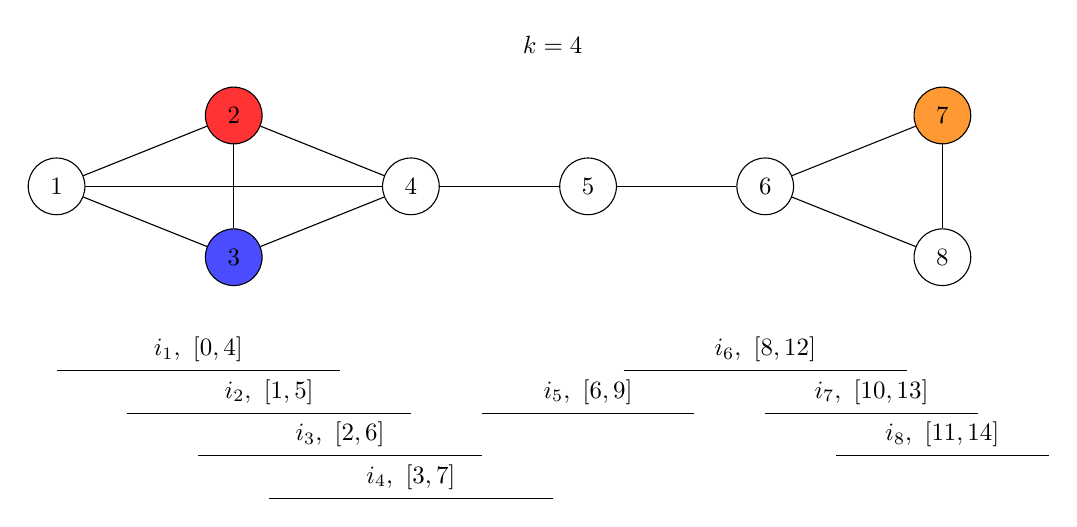
\begin{tikzpicture}[n/.style={circle,draw=black,minimum width=8mm}, scale=0.9, every
            node/.style={transform shape}]
            \node[n] (1) at (0,1) {$1$};
            \node[n,fill=red!80] (2) at (2.5,2) {$2$};
            \node[n,fill=blue!70] (3) at (2.5,0) {$3$};
            \node[n] (4) at (5,1) {$4$};
            \node[n] (5) at (7.5,1) {$5$};
            \node[n] (6) at (10,1) {$6$};
            \node[n,fill=orange!80] (7) at (12.5,2) {$7$};
            \node[n] (8) at (12.5,0) {$8$};

            \node (lab) at (7,3) {$k = 4$};

            \draw[-] (1) to (2);
            \draw[-] (1) to (3);
            \draw[-] (1) to (4);

            \draw[-] (2) to (3);
            \draw[-] (2) to (4);

            \draw[-] (3) to (4);

            \draw[-] (4) to (5);

            \draw[-] (5) to (6);

            \draw[-] (6) to (7);
            \draw[-] (6) to (8);
            
            \draw[-] (7) to (8);

            \draw[-] (0, -1.6) to node[above] {$i_1,\ [0,4]$} (4, -1.6);
            \draw[-] (1, -2.2) to node[above] {$i_2,\ [1,5]$} (5, -2.2);
            \draw[-] (2, -2.8) to node[above] {$i_3,\ [2,6]$} (6, -2.8);
            \draw[-] (3, -3.4) to node[above] {$i_4,\ [3,7]$} (7, -3.4);
            \draw[-] (6, -2.2) to node[above] {$i_5,\ [6,9]$} (9, -2.2);
            \draw[-] (8, -1.6) to node[above] {$i_6,\ [8,12]$} (12, -1.6);
            \draw[-] (10, -2.2) to node[above] {$i_7,\ [10, 13]$} (13, -2.2);
            \draw[-] (11, -2.8) to node[above] {$i_8,\ [11, 14]$} (14, -2.8);
        \end{tikzpicture}
    \end{center}
    \caption{Une instance de \precolor{} sur un graphe d'intervalles propre}
    \label{inst_precolor}
\end{figure}
% }}}

% {{{ FIGURES : Transformation
\begin{figure}
    \begin{center}
        % {{{ Precoloration
        \begin{minipage}[c][5cm][c]{0.35\linewidth}
            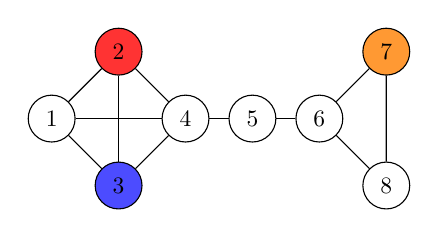
\begin{tikzpicture}[n/.style={circle,draw=black,minimum width=7mm},scale=0.85,every node/.style={transform shape}]
                \node[n] (1) at (0,1) {$1$};
                \node[n,fill=red!80] (2) at (1,2) {$2$};
                \node[n,fill=blue!70] (3) at (1,0) {$3$};
                \node[n] (4) at (2,1) {$4$};
                \node[n] (5) at (3,1) {$5$};
                \node[n] (6) at (4,1) {$6$};
                \node[n,fill=orange!80] (7) at (5,2) {$7$};
                \node[n] (8) at (5,0) {$8$};

                \draw[-] (1) to (2);
                \draw[-] (1) to (3);
                \draw[-] (1) to (4);

                \draw[-] (2) to (3);
                \draw[-] (2) to (4);

                \draw[-] (3) to (4);

                \draw[-] (4) to (5);

                \draw[-] (5) to (6);

                \draw[-] (6) to (7);
                \draw[-] (6) to (8);
                
                \draw[-] (7) to (8);
            \end{tikzpicture}
        \end{minipage}
        % }}}
        \hfill
        % {{{ Réservations
        \begin{minipage}[c][5cm][c]{0.55\linewidth}
            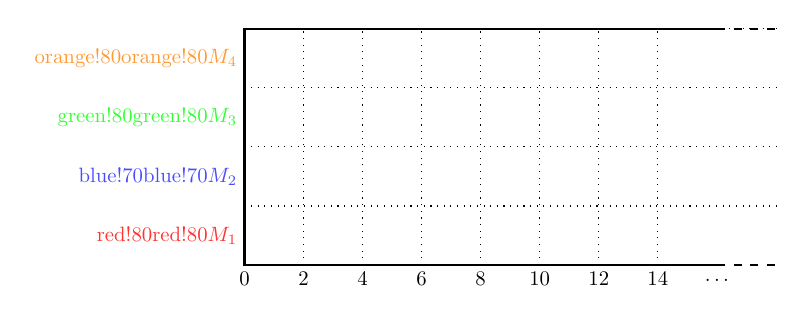
\begin{tikzpicture}[>=latex,scale=0.75,every node/.style={transform shape}]
                \pgfmathparse{2/14 * 7} \let\xpas\pgfmathresult
                \pgfmathparse{int(14/2)} \let\nbpas\pgfmathresult
                \pgfmathparse{\xpas/2} \let\unitxpas\pgfmathresult
                
                \draw[thick] (8,0) -- (0,0) -- (0,4) -- (8,4);
                \draw[thick,dashed] (8,0) -- (9,0);
                \draw[thick,dashed] (8,4) -- (9,4);

                \node[below] at (0, 0) {$0$};

                \foreach \x in {1,...,\nbpas}{
                    \pgfmathparse{\x * \xpas} \let\abscisse\pgfmathresult
                    \pgfmathparse{int(\x * 2)} \let\xlabel\pgfmathresult

                    \node[below] at (\abscisse, 0) {$\xlabel$};
                    \draw[dotted] (\abscisse,0) to (\abscisse,4);
                }

                \pgfmathparse{(\nbpas + 1) * \xpas} \let\abscisse\pgfmathresult
                \node[above] at (\abscisse, -0.4) {$\dots$};

                \foreach \y/\color in {1/red!80,2/blue!70,3/green!80,4/orange!80}{
                    \pgfmathparse{\y - 0.5} \let\ordlabel\pgfmathresult

                    \node[left, \color] at (0, \ordlabel) {$M_\y$};
                    \draw[dotted] (0, \y) to (9, \y);
                }

                \newresa{4}{1}{1}
                \newresa{4}{2}{2}
                \newresa{3}{4}{10}
            \end{tikzpicture}
        \end{minipage}
        % }}}

        % {{{ Coloration
        \begin{minipage}[c][5cm][c]{0.35\linewidth}
            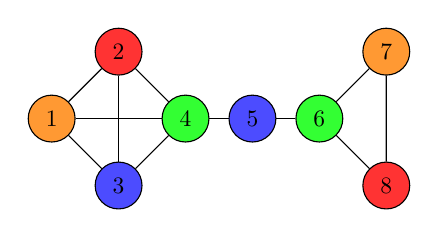
\begin{tikzpicture}[n/.style={circle,draw=black,minimum width=7mm},scale=0.85,every node/.style={transform shape}]
                \node[n,fill=orange!80] (1) at (0,1) {$1$};
                \node[n,fill=red!80] (2) at (1,2) {$2$};
                \node[n,fill=blue!70] (3) at (1,0) {$3$};
                \node[n,fill=green!80] (4) at (2,1) {$4$};
                \node[n,fill=blue!70] (5) at (3,1) {$5$};
                \node[n,fill=green!80] (6) at (4,1) {$6$};
                \node[n,fill=orange!80] (7) at (5,2) {$7$};
                \node[n,fill=red!80] (8) at (5,0) {$8$};

                \draw[-] (1) to (2);
                \draw[-] (1) to (3);
                \draw[-] (1) to (4);

                \draw[-] (2) to (3);
                \draw[-] (2) to (4);

                \draw[-] (3) to (4);

                \draw[-] (4) to (5);

                \draw[-] (5) to (6);

                \draw[-] (6) to (7);
                \draw[-] (6) to (8);
                
                \draw[-] (7) to (8);
            \end{tikzpicture}
        \end{minipage}
        % }}}
        \hfill
        % {{{ Ordonnancement
        \begin{minipage}[c][5cm][c]{0.55\linewidth}
            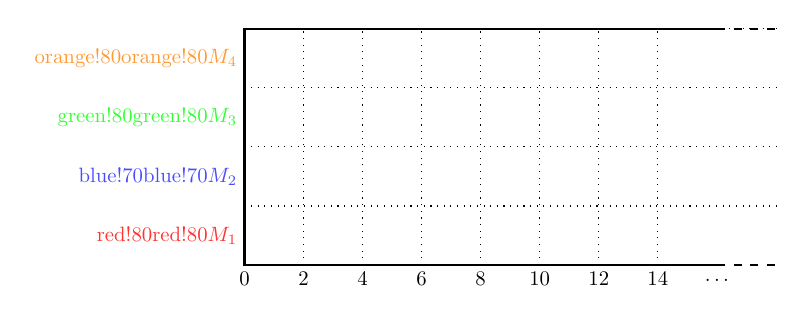
\begin{tikzpicture}[>=latex,scale=0.75,every node/.style={transform shape}]
                \pgfmathparse{2/14 * 7} \let\xpas\pgfmathresult
                \pgfmathparse{int(14/2)} \let\nbpas\pgfmathresult
                \pgfmathparse{\xpas/2} \let\unitxpas\pgfmathresult
                
                \draw[thick] (8,0) -- (0,0) -- (0,4) -- (8,4);
                \draw[thick,dashed] (8,0) -- (9,0);
                \draw[thick,dashed] (8,4) -- (9,4);

                \node[below] at (0, 0) {$0$};

                \foreach \x in {1,...,\nbpas}{
                    \pgfmathparse{\x * \xpas} \let\abscisse\pgfmathresult
                    \pgfmathparse{int(\x * 2)} \let\xlabel\pgfmathresult

                    \node[below] at (\abscisse, 0) {$\xlabel$};
                    \draw[dotted] (\abscisse,0) to (\abscisse,4);
                }

                \pgfmathparse{(\nbpas + 1) * \xpas} \let\abscisse\pgfmathresult
                \node[above] at (\abscisse, -0.4) {$\dots$};

                \foreach \y/\color in {1/red!80,2/blue!70,3/green!80,4/orange!80}{
                    \pgfmathparse{\y - 0.5} \let\ordlabel\pgfmathresult

                    \node[left, \color] at (0, \ordlabel) {$M_\y$};
                    \draw[dotted] (0, \y) to (9, \y);
                }

                \newresa{4}{1}{1}
                \newresa{4}{2}{2}
                \newresa{3}{4}{10}

                \newtask{4}{4}{0}
                \newtask{4}{3}{3}
                \newtask{3}{2}{6}
                \newtask{4}{3}{8}
                \newtask{3}{1}{11}

                \newhole{6}{1}{5}
                \newhole{1}{3}{7}
                \newhole{6}{4}{4}
            \end{tikzpicture}
        \end{minipage}
        % }}}
    \end{center}
    \caption{Illustration du principe de la transformation polynomiale}
    \label{fig_transpoly}
\end{figure}
% }}}
\end{ex}
% }}}

\subsection{La restriction du problème : \unitfischedpi{}}
\label{sspb_comp}

Considérons le problème~\ref{unitfischedpi} (p.~\pageref{unitfischedpi}), pour étudier sa
complexité, nous utiliserons à nouveau une réduction depuis \precolor{}, mais cette fois ci sur des
graphes d'intervalles propres tels que les intervalles ont même longueur et présentent des dates de
début et de fin sont entières.

\begin{nprop}
    Le problème \precolor{} sur les graphes d'intervalles de même longueur et dont les dates de début
    et de fin sont entières est équivalent au problème \precolor{} sur les graphes d'intervalles
    unitaires.
\end{nprop}

Un graphe d'intervalles propre étant équivalent à un graphe d'intervalles
unitaire~\cite{bogart1999short}, il est ensuite possible d'obtenir par dilatation un graphe
d'intervalles de même longueur ayant des dates de début et de fin entières.

\begin{ncorol}
    Le problème \precolor{} reste \textbf{NP}-complet sur la famille des graphes d'intervalles
    propres tels que les intervalles ont même longueur et présentent des datesd e début et de fin
    entières.
\end{ncorol}

\begin{nthrm}
    Le problème \unitfischedpi{} est \npc{}.
\end{nthrm}

% {{{ NP-COMPLETUDE : SECOND PROBLEME
Considérons une instance de \precolor{} sur un graphe d'intervalles caractérisée par un graphe $G =
(V,E)$, l'ensemble d'intervalles $\mathcal{I}$ associé, tel que tous les intervalles de
$\mathcal{I}$ ont la même taille et pour tout intervalle $i \in I$,
$\sint{i}$ et $\cint{i}$ sont entiers, un sous-ensembles de sommets $W \subseteq
V$ non vide et une coloration $c'$ qui à chaque sommet $w \in W$ associe une couleur. 

Nous pouvons construire une instance similaire\footnote{Possédant une solution si et seulement si
l'instance de départ possède une solution.} en multipliant les dates de début et de fin de chacun
des intervalles de $\mathcal{I}$ par $2$. Dans la mesure où il s'agit là d'une simple dilatation des
intervalles, le graphe défini par ce nouvel ensemble d'intervalle $\mathcal{I}'$ est isomorphe à
$G$.

Nous pouvons supposer que les dates de début et de fin des intervalles associés aux sommets de $G$
sont paires. 

La transformation se fait comme suit :
\begin{enumerate}
    \item À chaque couleur $i$, on associe une machine $M_i$, on a donc un ensemble $\mathcal{M}$ de
        $k$ machines.
    \item À chaque sommet $w \in W$, on associe une réservation unitaire $R_w$ sur la machine associée à
        la couleur de $w$ par la coloration $c'$ dont la date de début est donnée par le
        début de l'intervalle associé à $w$
        \[
            R_w = (M_{c'(w)}, [\sres{R_w} = \sint{i_w}, \cres{R_w} = \sres{R_w} + 1])
        \]
        Nous obtenons alors un ensemble de réservations $R = \{R_w : w \in W\}$.
    \item À chaque sommet $v \in V \backslash W$, on associe une tâche unitaire $T_v$ avec $\st{T_v}
        = \sint{i_v}$ et $\ct{T_v} = \st{T_v} + 1$. On a alors un ensemble de tâches $\mathcal{T} =
        \{T_v : v \in V \backslash W \}$.
    \item $z$ est défini comme la taille commune de chaque intervalle de $\mathcal{I}'$ moins $1$
        (la durée d'exécution d'une tâche unitaire).
\end{enumerate}
Cette transformation se fait en temps linéaire en le nombre de sommets de $G$ et donc en le nombre
d'événements.

Dans la mesure où le problème considéré est un spécification du problème \fischedpi{}, ce dernier
étant \npc{}, \unitfischedpi{} appartient donc à \textbf{NP}.

Mettons en évidence l'équivalence entre les deux problèmes :
\begin{bitemize}
    \item Supposons qu'il existe une coloration $c$ étendant $c'$ sur $G$, on peut obtenir un
        ordonnancement valide $\mathcal{O}$ en affectant à chaque événement $e_v$ associé au sommet
        $v \in V$, la machine correspondant à la couleur $c(v)$. Par définition de la coloration,
        deux sommets adjacents ont une couleur différente, et leur tâche associée\footnote{Les
        tâches sont concurrentes, puisque $G$ est un graphe d'intervalles.} s'exécutent sur des
        machines différentes, l'ordonnancement est donc valide. 

        De plus, le plus petit écart entre deux tâches non concurrentes est au moins égal à
        $z$ et ce par construction.
    \item Supposons maintenant qu'il existe un ordonnancement valide $\mathcal{O}$ dont le trou
        minimum est au moins égal à $z$, une coloration $c$ étendant $c'$ à $G$ peut être obtenue en
        associant à chaque sommet $v \in V$ la couleur correspondant à la machine sur laquelle est
        exécutée l'événement $e_v$.

        De la même manière que précédemment raisonnons par l'absurde pour démontrer la validité de
        la coloration. Supposons qu'il existe un ordonnancement valide, tel que le trou minimum est
        au moins égal à $z$ et tel que deux sommets adjacents $u$ et $v$ ont même couleur par la
        transformation précédente. Si $u$ et $v$ ont même couleur, ils s'exécutent sur la même
        machine. Le trou séparant $T_u$ et $T_v$ est par hypothèse supérieur ou égal à $z$, de plus
        $u$ et $v$ étant adjacents, les intervalles $i_u$ et $i_v$ s'intersectent. Or, $\sint{i_u} =
        \st{T_u}$ et $\sint{i_v} = \st{T_v}$ et donc $\pint{i_u} > z+1$ ou $\pint{i_v} > z+1$.
        Contradiction.
\end{bitemize}

Le problème \unitfischedpi{} appartenant à \textbf{NP}, la transformation étant polynomiale, alors
\unitfischedpi{} est \npc{}.
% }}}

\begin{ex}
    Considérons l'instance du problème de la figure~\ref{precol_supgraph}\footnote{Notons qu'il
    s'agit de l'instance étudiée précédemment avec des intervalles de même longueur.}, nous dilatons
    cette instance afin d'obtenir les intervalles de la figure~\ref{precol_supgraph_pair} à valeur
    entières et paires. La réduction est illustrée à la figure~\ref{fig_transpoly_bis}.

    Comme précédemment, on cherche à déterminer si le graphe est $4-$colorable, on utilise donc
    quatre machines, on crée une réservation unitaire pour chaque sommet précoloré, puis on crée une
    tâche unitaire pour chaque sommet non précoloré.

    On calcule la valeur de $z$, ici $z = 8 - 1 = 7$. L'ordonnancement donné est un ordonnancement
    valide dont le trou minimum est égal à $z$ et comme on peut le voir, il définit une coloration
    $c$ valide étendant la précoloration sur $G$.

% {{{ FIGURES : NP-COMPLETUDE
% {{{ FIGURE : Instance
\begin{figure}
    \begin{center}
        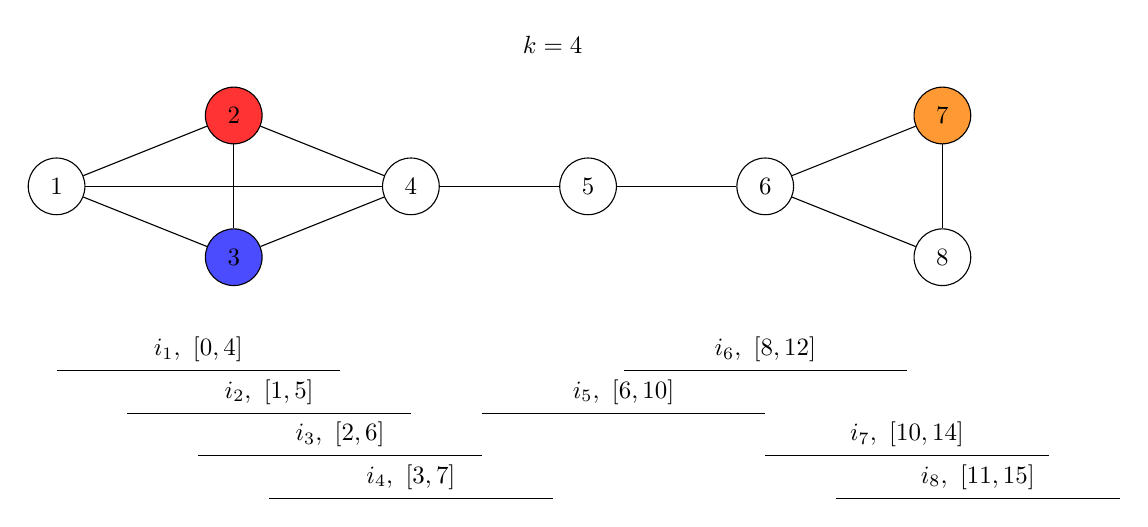
\begin{tikzpicture}[n/.style={circle,draw=black,minimum width=8mm}, scale=0.9, every
            node/.style={transform shape}]
            \node[n] (1) at (0,1) {$1$};
            \node[n,fill=red!80] (2) at (2.5,2) {$2$};
            \node[n,fill=blue!70] (3) at (2.5,0) {$3$};
            \node[n] (4) at (5,1) {$4$};
            \node[n] (5) at (7.5,1) {$5$};
            \node[n] (6) at (10,1) {$6$};
            \node[n,fill=orange!80] (7) at (12.5,2) {$7$};
            \node[n] (8) at (12.5,0) {$8$};

            \node (lab) at (7,3) {$k = 4$};

            \draw[-] (1) to (2);
            \draw[-] (1) to (3);
            \draw[-] (1) to (4);

            \draw[-] (2) to (3);
            \draw[-] (2) to (4);

            \draw[-] (3) to (4);

            \draw[-] (4) to (5);

            \draw[-] (5) to (6);

            \draw[-] (6) to (7);
            \draw[-] (6) to (8);
            
            \draw[-] (7) to (8);

            \draw[-] (0, -1.6) to node[above] {$i_1,\ [0,4]$} (4, -1.6);
            \draw[-] (1, -2.2) to node[above] {$i_2,\ [1,5]$} (5, -2.2);
            \draw[-] (2, -2.8) to node[above] {$i_3,\ [2,6]$} (6, -2.8);
            \draw[-] (3, -3.4) to node[above] {$i_4,\ [3,7]$} (7, -3.4);
            \draw[-] (6, -2.2) to node[above] {$i_5,\ [6,10]$} (10, -2.2);
            \draw[-] (8, -1.6) to node[above] {$i_6,\ [8,12]$} (12, -1.6);
            \draw[-] (10, -2.8) to node[above] {$i_7,\ [10, 14]$} (14, -2.8);
            \draw[-] (11, -3.4) to node[above] {$i_8,\ [11, 15]$} (15, -3.4);
        \end{tikzpicture}
    \end{center}
    \caption{Une instance de \precolor{} sur un graphe d'intervalles de même longueur à valeurs
    entières}
    \label{precol_supgraphe}
\end{figure}
% }}}

% {{{ FIGURE : Instance Paire
\begin{figure}
    \begin{center}
        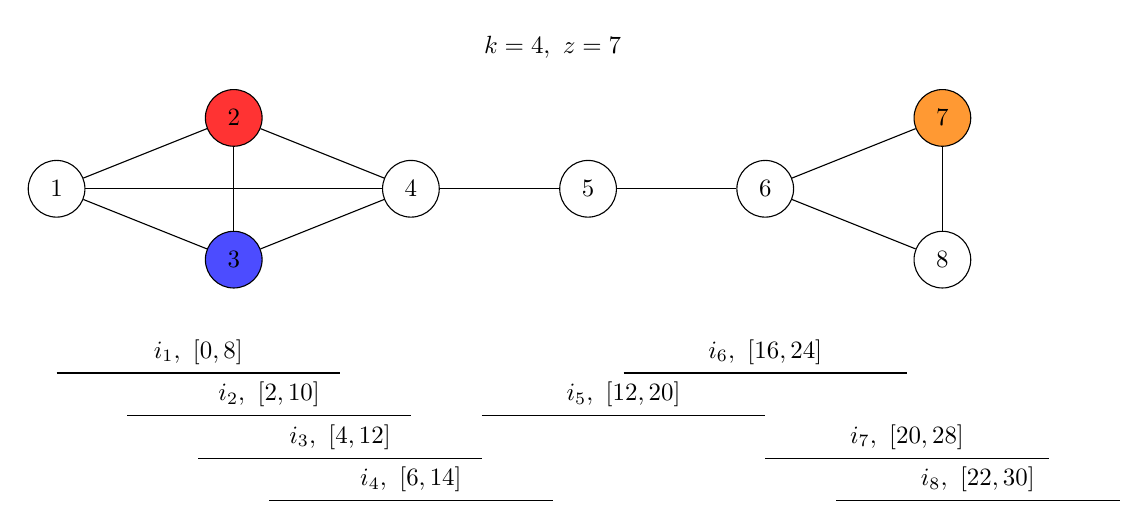
\begin{tikzpicture}[n/.style={circle,draw=black,minimum width=8mm}, scale=0.9, every
            node/.style={transform shape}]
            \node[n] (1) at (0,1) {$1$};
            \node[n,fill=red!80] (2) at (2.5,2) {$2$};
            \node[n,fill=blue!70] (3) at (2.5,0) {$3$};
            \node[n] (4) at (5,1) {$4$};
            \node[n] (5) at (7.5,1) {$5$};
            \node[n] (6) at (10,1) {$6$};
            \node[n,fill=orange!80] (7) at (12.5,2) {$7$};
            \node[n] (8) at (12.5,0) {$8$};

            \node (lab) at (7,3) {$k = 4,\ z = 7$};

            \draw[-] (1) to (2);
            \draw[-] (1) to (3);
            \draw[-] (1) to (4);

            \draw[-] (2) to (3);
            \draw[-] (2) to (4);

            \draw[-] (3) to (4);

            \draw[-] (4) to (5);

            \draw[-] (5) to (6);

            \draw[-] (6) to (7);
            \draw[-] (6) to (8);
            
            \draw[-] (7) to (8);

            \draw[-] (0, -1.6) to node[above] {$i_1,\ [0,8]$} (4, -1.6);
            \draw[-] (1, -2.2) to node[above] {$i_2,\ [2,10]$} (5, -2.2);
            \draw[-] (2, -2.8) to node[above] {$i_3,\ [4,12]$} (6, -2.8);
            \draw[-] (3, -3.4) to node[above] {$i_4,\ [6,14]$} (7, -3.4);
            \draw[-] (6, -2.2) to node[above] {$i_5,\ [12,20]$} (10, -2.2);
            \draw[-] (8, -1.6) to node[above] {$i_6,\ [16,24]$} (12, -1.6);
            \draw[-] (10, -2.8) to node[above] {$i_7,\ [20, 28]$} (14, -2.8);
            \draw[-] (11, -3.4) to node[above] {$i_8,\ [22, 30]$} (15, -3.4);
        \end{tikzpicture}
    \end{center}
    \caption{Une instance de \precolor{} sur un graphe d'intervalles de même longueur à valeurs
    entières et paires}
    \label{paire_precol_supgraphe}
\end{figure}
% }}}

% {{{ FIGURES : Transformation
\begin{figure}
    \begin{center}
        % {{{ Precoloration
        \begin{minipage}[c][5cm][c]{0.35\linewidth}
            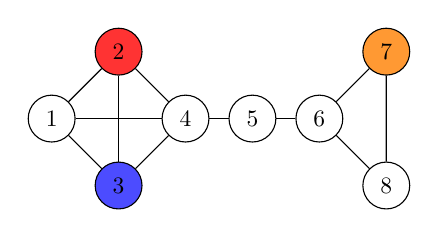
\begin{tikzpicture}[n/.style={circle,draw=black,minimum width=7mm},scale=0.85,every node/.style={transform shape}]
                \node[n] (1) at (0,1) {$1$};
                \node[n,fill=red!80] (2) at (1,2) {$2$};
                \node[n,fill=blue!70] (3) at (1,0) {$3$};
                \node[n] (4) at (2,1) {$4$};
                \node[n] (5) at (3,1) {$5$};
                \node[n] (6) at (4,1) {$6$};
                \node[n,fill=orange!80] (7) at (5,2) {$7$};
                \node[n] (8) at (5,0) {$8$};

                \draw[-] (1) to (2);
                \draw[-] (1) to (3);
                \draw[-] (1) to (4);

                \draw[-] (2) to (3);
                \draw[-] (2) to (4);

                \draw[-] (3) to (4);

                \draw[-] (4) to (5);

                \draw[-] (5) to (6);

                \draw[-] (6) to (7);
                \draw[-] (6) to (8);
                
                \draw[-] (7) to (8);
            \end{tikzpicture}
        \end{minipage}
        % }}}
        \hfill
        % {{{ Réservations
        \begin{minipage}[c][5cm][c]{0.55\linewidth}
            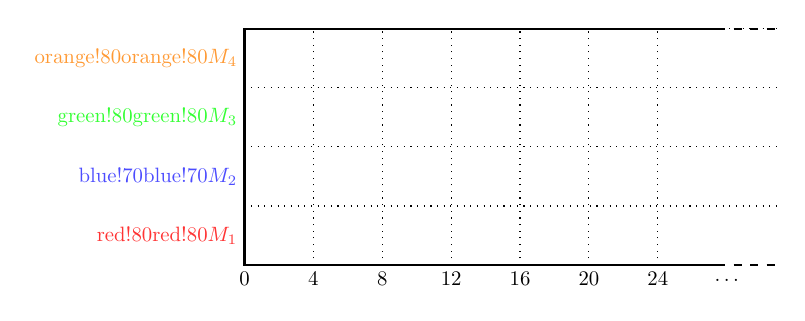
\begin{tikzpicture}[>=latex,scale=0.75,every node/.style={transform shape}]
                \pgfmathparse{4/24 * 7} \let\xpas\pgfmathresult
                \pgfmathparse{int(24/4)} \let\nbpas\pgfmathresult
                \pgfmathparse{\xpas/4} \let\unitxpas\pgfmathresult
                
                \draw[thick] (8,0) -- (0,0) -- (0,4) -- (8,4);
                \draw[thick,dashed] (8,0) -- (9,0);
                \draw[thick,dashed] (8,4) -- (9,4);

                \node[below] at (0, 0) {$0$};

                \foreach \x in {1,...,\nbpas}{
                    \pgfmathparse{\x * \xpas} \let\abscisse\pgfmathresult
                    \pgfmathparse{int(\x * 4)} \let\xlabel\pgfmathresult

                    \node[below] at (\abscisse, 0) {$\xlabel$};
                    \draw[dotted] (\abscisse,0) to (\abscisse,4);
                }

                \pgfmathparse{(\nbpas + 1) * \xpas} \let\abscisse\pgfmathresult
                \node[above] at (\abscisse, -0.4) {$\dots$};

                \foreach \y/\color in {1/red!80,2/blue!70,3/green!80,4/orange!80}{
                    \pgfmathparse{\y - 0.5} \let\ordlabel\pgfmathresult

                    \node[left, \color] at (0, \ordlabel) {$M_\y$};
                    \draw[dotted] (0, \y) to (9, \y);
                }

                \newresa{1}{1}{2}
                \newresa{1}{2}{4}
                \newresa{1}{4}{20}
            \end{tikzpicture}
        \end{minipage}
        % }}}

        % {{{ Coloration
        \begin{minipage}[c][5cm][c]{0.35\linewidth}
            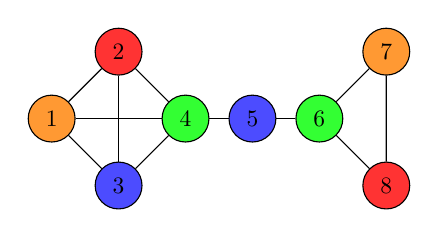
\begin{tikzpicture}[n/.style={circle,draw=black,minimum width=7mm},scale=0.85,every node/.style={transform shape}]
                \node[n,fill=orange!80] (1) at (0,1) {$1$};
                \node[n,fill=red!80] (2) at (1,2) {$2$};
                \node[n,fill=blue!70] (3) at (1,0) {$3$};
                \node[n,fill=green!80] (4) at (2,1) {$4$};
                \node[n,fill=blue!70] (5) at (3,1) {$5$};
                \node[n,fill=green!80] (6) at (4,1) {$6$};
                \node[n,fill=orange!80] (7) at (5,2) {$7$};
                \node[n,fill=red!80] (8) at (5,0) {$8$};

                \draw[-] (1) to (2);
                \draw[-] (1) to (3);
                \draw[-] (1) to (4);

                \draw[-] (2) to (3);
                \draw[-] (2) to (4);

                \draw[-] (3) to (4);

                \draw[-] (4) to (5);

                \draw[-] (5) to (6);

                \draw[-] (6) to (7);
                \draw[-] (6) to (8);
                
                \draw[-] (7) to (8);
            \end{tikzpicture}
        \end{minipage}
        % }}}
        \hfill
        % {{{ Ordonnancement
        \begin{minipage}[c][5cm][c]{0.55\linewidth}
            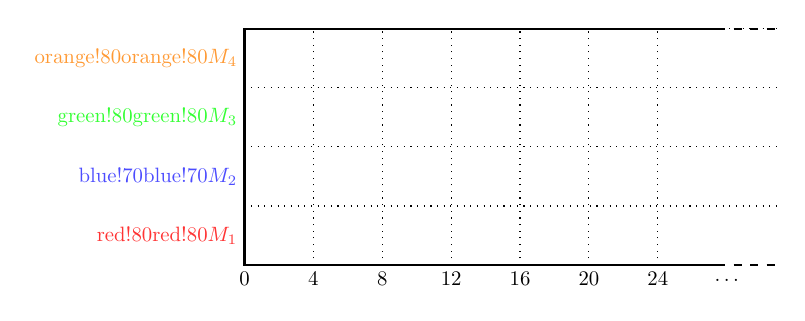
\begin{tikzpicture}[>=latex,scale=0.75,every node/.style={transform shape}]
                \pgfmathparse{4/24 * 7} \let\xpas\pgfmathresult
                \pgfmathparse{int(24/4)} \let\nbpas\pgfmathresult
                \pgfmathparse{\xpas/4} \let\unitxpas\pgfmathresult
                
                \draw[thick] (8,0) -- (0,0) -- (0,4) -- (8,4);
                \draw[thick,dashed] (8,0) -- (9,0);
                \draw[thick,dashed] (8,4) -- (9,4);

                \node[below] at (0, 0) {$0$};

                \foreach \x in {1,...,\nbpas}{
                    \pgfmathparse{\x * \xpas} \let\abscisse\pgfmathresult
                    \pgfmathparse{int(\x * 4)} \let\xlabel\pgfmathresult

                    \node[below] at (\abscisse, 0) {$\xlabel$};
                    \draw[dotted] (\abscisse,0) to (\abscisse,4);
                }

                \pgfmathparse{(\nbpas + 1) * \xpas} \let\abscisse\pgfmathresult
                \node[above] at (\abscisse, -0.4) {$\dots$};

                \foreach \y/\color in {1/red!80,2/blue!70,3/green!80,4/orange!80}{
                    \pgfmathparse{\y - 0.5} \let\ordlabel\pgfmathresult

                    \node[left, \color] at (0, \ordlabel) {$M_\y$};
                    \draw[dotted] (0, \y) to (9, \y);
                }

                \newresa{1}{1}{2}
                \newresa{1}{2}{4}
                \newresa{1}{4}{20}

                \newtask{1}{4}{0}
                \newtask{1}{3}{6}
                \newtask{1}{2}{12}
                \newtask{1}{3}{16}
                \newtask{1}{1}{22}

                \newhole{19}{1}{3}
                \newhole{7}{2}{5}
                \newhole{9}{3}{7}
                \newhole{19}{4}{1}
            \end{tikzpicture}
        \end{minipage}
        % }}}
    \end{center}
    \caption{Illustration du principe de la transformation polynomiale}
    \label{fig_transpoly_bis}
\end{figure}
% }}}
% }}}
\end{ex}
% }}}

